\documentclass[12pt]{article}
 
\usepackage[margin=1in]{geometry} 
\usepackage[utf8]{inputenc}
\usepackage{polski} 
\usepackage{hyperref}
\usepackage{graphicx}
\setlength{\parindent}{0pt}
\setlength{\parskip}{7.5pt}

\title{%
Elektroniczna szachownica z komputerem szachowym \\
\large Przypadki użycia
}
\author{Gabriel Wechta (250111),\\ Patryk Majewski (250134) }
\date{}

\begin{document}
\maketitle

\section{Rozpoczęcie rozgrywki z graczem lub z komputerem}
\textbf{Priorytet:} wysoki

\textbf{Aktor podstawowy:} Gracz 1

\textbf{Typ opisu:} szczegółowy

\textbf{Udziałowcy i cele:} 

Uczestniczą: Gracz 1, Gracz 2 oraz Silnik Szachowy. Jest to podstawowy przypadek użycia urządzenia, rozpoczyna on wszystkie procesy służące do rejestracji oraz walidacji ruchów i sytuacji na szachownicy. Istnieją dwie przypadki przebiegu tego PU: M - rozpoczęcie rozgrywki gdzie przeciwnikiem jest inny żywy gracz (Gracz 2), S - przeciwnikiem jest komputer (Silnik Szachowy).

\textbf{Wyzwalacz:} Przycisk Play/Pause.

\textbf{Typ wyzwalacza:} zewnętrzny

\textbf{Powiązania:} Uruchamia wszystkie procesy służące do rejestracji rozgrywki. 
\begin{itemize}
	\item Asocjacja: PU: 5, 7, 9, 10, 11.
	\item Zawieranie: PU 6.
	\item Rozszerzenia: 
	\item Generalizacja:
\end{itemize} 

\textbf{Zwykły przepływ zdarzeń:}  
\begin{enumerate}
\item Wciśnięcie przycisku Play/Pause.
\item Komunikacja z Silnikiem Szachowym aby rozpoczął rejestrację inputu z szachownicy.
\item W dalszej części działania systemu już poza PU, w zależności od trybu gry:
\begin{itemize}
    \item M -- Silnik Szachowy prowadzi walidacje ruchów spodziewając się ruchów po obu stronach szachownicy.
    \item S -- Silnik Szachowy poza walidacją ruchów komunikuje też swoje ruchu.
\end{itemize}
\item PU kończy działanie gdy interfejs pomiędzy szachownicą a Silnikiem Szachowym zacznie nasłuchiwać. 
\end{enumerate}
% \textbf{Przepływy poboczne:}

\textbf{Przepływy alternatywne/wyjątkowe:}
\begin{enumerate}
\item Wykrycie złego ustawienia bierek w pozycji startowej.
\item Wyświetlenie informacji o złym ustawieniu bierek.
\end{enumerate}

\section{Wykonanie ruchu w imieniu gracza}
\textbf{Priorytet:} wysoki

\textbf{Aktor podstawowy:} Gracz 1 albo Gracz 2

\textbf{Typ opisu:} szczegółowy

\textbf{Udziałowcy i cele:} 

Uczestniczą: Gracz 1, Gracz 2, Silnik Szachowy. Celem jest wykonanie przez użytkowników poprawnego ruchu szachowego. Gracz 1 i Gracz 2 fizycznie wykonują ruchy na szachownicy, Silnik Szachowy jest odpowiedzialny za ewaluację i zapis sytuacji na szachownicy i w przypadku niepoprawnego przepływu wyłapanie go i zaalarmowanie użytkowników. 

\textbf{Wyzwalacz:} Przesunięcie bierki na szachownicy.

\textbf{Typ wyzwalacza:} zewnętrzny

\textbf{Powiązania:} Jest oceniana jego poprawność jak i jego jakość.
	\begin{itemize}\item Asocjacja: PU: 4, 7, 8, 9, 10, 11.
	\item Zawieranie: 
	\item Rozszerzenia: w przypadku ruchu kończącego rozgrywkę realizowane jest PU 4.
	\item Generalizacja: 
\end{itemize} 
\textbf{Zwykły przepływ zdarzeń:}  
\begin{enumerate}
\item Jeden z Graczy podnosi bierkę i przedstawia ją na pole, na którym chce aby bierka się znalazła.
\item Sprawdzenie legalności ruchu bierką.
\item Zatrzymanie zegara gracza wykonującego ruch.
\item Zapisanie ruchu bierką.
\item Ewaluacja ruchu bierką.
\item Zapis ruchu w notacji szachowej jest wyświetlany na wyświetlaczu.
\end{enumerate} 

\textbf{Przepływy poboczne:}

W przypadku podniesienia bierki i odstawienia jej na to samo pole na którym stała:
\begin{enumerate}
\item Wznowienie zegara gracza wykonującego ruch.
\item Oczekiwanie pełnego legalnego ruchu.
\end{enumerate}

\textbf{Przepływy alternatywne/wyjątkowe:}
\begin{enumerate}

\item Przypadek zgłoszenia błędu ustawienia bierek przez PU 10:
\begin{enumerate}
\item Wyświetlenie zależnej od błędu informacji na wyświetlaczu.
\item Zatrzymanie zegara gracza wykonującego ruch.
\item Zaniechanie odczytywania ruchów do momentu powrócenia do ostatniej legalnej, zarejestrowanej pozycji.
\end{enumerate}

\item Przypadek zgłoszenia nielegalności ruchu przez PU 9:
\begin{enumerate}
\item Wyświetlenie informacji na wyświetlaczu.
\item Zatrzymanie zegara gracza wykonującego ruch.
\item Zaniechanie odczytywania ruchów do momentu powrócenia do ostatniej legalnej, zarejestrowanej pozycji.
\end{enumerate}
\end{enumerate}



\section{Wykonanie ruchu w imieniu komputera}

\textbf{Priorytet:} wysoki

\textbf{Aktor podstawowy:} Gracz 1

\textbf{Typ opisu:} szczegółowy

\textbf{Udziałowcy i cele:} 

Uczestniczą: Gracz 1, Silnik Szachowy. Celem jest wykonanie przez użytkownika ruchu szachowego. Może to być ruch zgłoszony przez Silnik Szachowy, albo dowolny inny legalny ruch. Gracz 1 fizycznie wykonuje ruch na szachownicy. Silnik Szachowy, niezależnie czy zgłoszony wcześniej przez niego ruch został wykonany, przeprowadza ewaluację i zapis sytuacji na szachownicy. W przypadku niepoprawnego przepływu ruchu alarmuje użytkownika. 

\textbf{Wyzwalacz:} Przesunięcie bierki na szachownicy.

\textbf{Typ wyzwalacza:} zewnętrzny

\textbf{Powiązania:} Jest to realizacja ruchu zgłoszonego przez Silnik Szachowy, który zależy od PU 5.
	\begin{itemize}
	\item Asocjacja: PU: 4, 5, 7, 8, 9, 10, 11, 12.
	\item Zawieranie: 
	\item Rozszerzenia: w przypadku ruchu kończącego rozgrywkę realizowane jest PU 4.
	\item Generalizacja: 
\end{itemize} 

\textbf{Zwykły przepływ zdarzeń:}  
\begin{enumerate}
\item Użytkownik podnosi bierkę i przedstawia ją na pole, które wskazał Silnik Szachowy.
\item Sprawdzenie legalności ruchu bierką.
\item Zapisanie ruchu bierką.
\item Ewaluacja ruchu bierką.
\item Zapis ruchu w notacji szachowej jest wyświetlany na wyświetlaczu.
\end{enumerate} 

\textbf{Przepływy poboczne:}
\begin{enumerate}
\item Przypadek wykonaniu ruchu innego niż ten wskazany przez Silnik Szachowy:
\item Sprawdzenie legalności ruchu bierką.
\item Zapisanie ruchu bierką.
\item Adaptacja Silnika Szachowego do przeprowadzonego ruchu. Realizowana przez PU 12.
\item Zapis ruchu w notacji szachowej jest wyświetlany na wyświetlaczu.
\end{enumerate}

\textbf{Przepływy alternatywne/wyjątkowe:}

Jak w PU 2.
\begin{enumerate}
\item Przypadek zgłoszenia błędu ustawienia bierek przez PU 10:
    \begin{enumerate}
    \item Wyświetlenie zależnej od błędu informacji na wyświetlaczu.
    \item Zaniechanie odczytywania ruchów do momentu powrócenia do ostatniej \item legalnej, zarejestrowanej pozycji.
    \end{enumerate}
\item Przypadek zgłoszenia nielegalności ruchu przez PU 9:
    \begin{enumerate}
    \item Wyświetlenie informacji na wyświetlaczu.
    \item Zaniechanie odczytywania ruchów do momentu powrócenia do ostatniej legalnej, zarejestrowanej pozycji.
    \end{enumerate}
\end{enumerate}



\section{Zakończenie partii}

\textbf{Priorytet:} wysoki

\textbf{Aktor podstawowy:} Silnik szachowy

\textbf{Typ opisu:} ogólny

\textbf{Udziałowcy i cele:} 
Uczestniczą: Gracz 1, Silnik Szachowy i ewentualnie Gracz 2. Po wykonaniu ruchu matującego lub patujacego wykrytego przez PU 8 lub po upływie ustalonego w PU 5 czasu wyświetlane są informacje o zakończeniu partii.

\textbf{Wyzwalacz:} Zapisany ruch lub zegar.

\textbf{Typ wyzwalacza:} wewnętrzny

\textbf{Powiązania:} Jest to ostatni element w naturalnym przebiegu życia systemu.
	\begin{itemize}\item Asocjacja: PU: 2, 3.
	\item Zawieranie: 
	\item Rozszerzenia: PU 2, 3.
	\item Generalizacja: 
\end{itemize} 

\textbf{Zwykły przepływ zdarzeń:}  
\begin{enumerate}
\item Wyświetlenie informacji o wyniku partii, w formacie kto wygrał, w jaki sposób, jaki był stan zegarów.
\end{enumerate} 

% \textbf{Przepływy poboczne:}

% \textbf{Przepływy alternatywne/wyjątkowe:}



\section{Wybranie poziomu trudności, koloru bierek i czasu}

\textbf{Priorytet:} średni

\textbf{Aktor podstawowy:} Gracz 1

\textbf{Typ opisu:} ogólny

\textbf{Udziałowcy i cele:} 

Uczestniczą: Gracz 1, Silnik Szachowy. Celem jest wybór parametrów partii szachowej. Gdy partia jest rozgrywana między dwoma graczami nie ma możliwości wyboru poziomu trudności i koloru bierek. Wybór poziomu trudności wpływa na styl gry komputera, tj które z najlepszych posunięć wybierze przy wykonywania swojego ruchu i ile czasu z zegara upłynie zanim go wykona. 

\textbf{Wyzwalacz:} Wybranie opcji z menu.

\textbf{Typ wyzwalacza:} zewnętrzny

\textbf{Powiązania:} Wpływa na PU 8.
	\begin{itemize}\item Asocjacja: PU: 3, 4, 8.
	\item Zawieranie: 
	\item Rozszerzenia:
	\item Generalizacja: 
\end{itemize} 

\textbf{Zwykły przepływ zdarzeń:}  
\begin{enumerate}
\item Użytkownik wybiera odpowiednie pole z menu.
\item Użytkownik wybiera odpowiednie pola z submenu.
\end{enumerate} 

% \textbf{Przepływy poboczne:}

% \textbf{Przepływy alternatywne/wyjątkowe:}



\section{Wznowienie gry od wybranej pozycji}

\textbf{Priorytet:} średni

\textbf{Aktor podstawowy:} Gracz 1

\textbf{Typ opisu:} szczegółowy

\textbf{Udziałowcy i cele:} 

Uczestniczą: Gracz 1, Silnik Szachowy. Po wybraniu odpowiedniej opcji użytkownik może ustawić bierki w wybranej przez siebie pozycji i wznowić grę od tego momentu.

\textbf{Wyzwalacz:} Wybranie opcji z menu.

\textbf{Typ wyzwalacza:} zewnętrzny

\textbf{Powiązania:} Takie same jak w przypadku rozgrywania normalnej partii.
	\begin{itemize}\item Asocjacja: PU: 2, 3, 4, 5, 7, 8, 9, 10, 11, 12.
	\item Zawieranie: 
	\item Rozszerzenia:
	\item Generalizacja:
\end{itemize} 

\textbf{Zwykły przepływ zdarzeń:} 
\begin{enumerate}
\item Wybranie opcji z menu.
\item Ustawienie bierek na szachownicy.
\item Wciśnięcie przycisku Play/Pause.
\item Komunikacja z Silnikiem Szachowym aby rozpoczął rejestrację inputu z szachownicy.
\item W dalszej części działania systemu już poza PU, w zależności od trybu gry:
    \begin{itemize}
    \item M -- Silnik Szachowy prowadzi walidacje ruchów spodziewając się ruchów po obu stronach szachownicy.
    \item S -- Silnik Szachowy poza walidacją ruchów komunikuje też swoje ruchu.
    \end{itemize}
\item PU kończy działanie gdy interfejs pomiędzy szachownicą a Silnikiem Szachowym zacznie nasłuchiwać. 
\end{enumerate} 

% \textbf{Przepływy poboczne:}

\textbf{Przepływy alternatywne/wyjątkowe:}
\begin{enumerate}
    \item W przypadku wykrycia złego ustawienia bierek w pozycji startowej przez PU 10:
    \begin{enumerate}
        \item Wyświetlenie informacji o złym ustawieniu bierek.
    \end{enumerate}
    \item W przypadku wznowienia partii z wcześniej zapisanej przed wyłączeniem urządzenia:
    \begin{enumerate}
        \item Wczytanie zapisanej partii do Silnika Szachowego.
        \item Wyświetlanie jej na wyświetlaczu.
        \item Oczekiwanie na ustawienie bierek na szachownicy.
    \end{enumerate}
\end{enumerate}



\section{Zapisanie stanu partii}

\textbf{Priorytet:} wysoki

\textbf{Aktor podstawowy:} Silnik Szachowy

\textbf{Typ opisu:} szczegółowy

\textbf{Udziałowcy i cele:} 

Uczestniczy: Silnik Szachowy. PU jest realizowane za każdym razem gdy następuje zmiana na szachownicy. Celem PU jest przeprowadzenie odczytu z czujników zamieszczonych na szachownicy aby dostać zapis stanu, który posłuży następnie do przeprowadzenia PU 8, PU 9 i ewentualnie PU 3 i PU 12. 

\textbf{Wyzwalacz:} Szachownica.

\textbf{Typ wyzwalacza:} zewnętrzny

\textbf{Powiązania:} Zapis stanu partii stanowi źródło informacji o obecnym stanie partii dla PU 3, 8, 9 i 12.
	\begin{itemize}\item Asocjacja: PU: 2, 3, 4, 5, 6, 8, 9, 10, 11, 12.
	\item Zawieranie: 
	\item Rozszerzenia:
	\item Generalizacja:
\end{itemize} 

\textbf{Zwykły przepływ zdarzeń:}  
\begin{enumerate}
\item Wykrycie zmiany przez czujniki.
\item Odczyt z czujników.
\item Mapowanie ciężaru na bierki.
\item Dodanie ruchu do obecnego zapisu partii.
\end{enumerate} 

\textbf{Przepływy poboczne:}

W przypadku PU 6, zapis zaczyna się od “,,,” oznaczających “nieznany przebieg partii do tego momentu”.

\textbf{Przepływy alternatywne/wyjątkowe:}
\begin{enumerate}
\item W przypadku niejednoznacznego odczytu z czujników:
    \begin{enumerate}
    \item Wykrycie zmiany przez czujniki.
    \item Odczyt z czujników.
    \item Mapowanie ciężaru na bierki.
    \item Wykrycie niejednoznaczności.
    \item Wyświetlenie prośby o poprawienie ustawienia bierek.
    \end{enumerate}
\item W przypadku wyłączenia szachownicy:
    \begin{enumerate}
    \item Zapisanie ostatniego stanu gry w pamięci urządzenia.
    \end{enumerate}
\end{enumerate}



\section{Szukanie najlepszych ruchów w pozycji}

\textbf{Priorytet:} wysoki

\textbf{Aktor podstawowy:} Silnik Szachowy

\textbf{Typ opisu:} ogólny

\textbf{Udziałowcy i cele:} 

Uczestniczy: Silnik Szachowy. PU jest realizowane za każdym razem gdy następuje zmiana na szachownicy. Celem PU jest znalezienie najlepszych ruchów w pozycji na podstawie obecnego położenia bierek, PU 7. PU używa do tego implementacji silnika szachowego.

\textbf{Wyzwalacz:} Interfejs zapisu stanu rozgrywki.

\textbf{Typ wyzwalacza:} wewnętrzny

\textbf{Powiązania:} PU korzysta z danych dostarczonych mu przez PU 7. Jest niezbędne dla PU 3 i PU 12.
	\begin{itemize}\item Asocjacja: PU: 7, 3, 12.
	\item Zawieranie: 
	\item Rozszerzenia:
	\item Generalizacja:
\end{itemize} 

\textbf{Zwykły przepływ zdarzeń:}  
\begin{enumerate}
\item Otrzymanie obecnego stanu partii.
\item Obliczenie najlepszych ruchów w pozycji.
\item Wyświetlenie na ekranie podpowiedzi w postaci najbardziej korzystnych dla gracza ruchów.
\end{enumerate} 

% \textbf{Przepływy poboczne:}

% \textbf{Przepływy alternatywne/wyjątkowe:}



\section{Sprawdzenie legalności ruchu}

\textbf{Priorytet:} wysoki

\textbf{Aktor podstawowy:} Silnik Szachowy

\textbf{Typ opisu:} ogólny

\textbf{Udziałowcy i cele:} 

Uczestniczą: Silnik Szachowy. Analiza czy ruch był zgodny z regułami gry w szachy.

\textbf{Wyzwalacz:} Interfejs zapisu stanu rozgrywki.

\textbf{Typ wyzwalacza:} wewnętrzny

\textbf{Powiązania:} 
	\begin{itemize}\item Asocjacja: PU: 7, 11.
	\item Zawieranie: 
	\item Rozszerzenia:
	\item Generalizacja:
\end{itemize} 
\textbf{Zwykły przepływ zdarzeń:}  
\begin{enumerate}
\item Otrzymanie obecnego stanu partii.
\item Analiza legalności ruchu.
\item Wywołanie PU 11.
\end{enumerate} 

% \textbf{Przepływy poboczne:}

% \textbf{Przepływy alternatywne/wyjątkowe:}



\section{Sprawdzenie ustawienia bierek}

\textbf{Priorytet:} wysoki

\textbf{Aktor podstawowy:} Silnik Szachowy

\textbf{Typ opisu:} ogólny

\textbf{Udziałowcy i cele:} 

Uczestniczą: Silnik Szachowy. Analiza czy bierki nie zostały przemieszczone w nieodpowiednim momencie lub czy nie zostały strącone.

\textbf{Wyzwalacz:} Szachownica.

\textbf{Typ wyzwalacza:} zewnętrzny

\textbf{Powiązania:} 
	\begin{itemize}\item Asocjacja: PU 11.
	\item Zawieranie: 
	\item Rozszerzenia:
	\item Generalizacja:
\end{itemize} 

\textbf{Zwykły przepływ zdarzeń:}  
\begin{enumerate}
\item Wykrycie zmiany przez czujniki.
\item Odczyt z czujników.
\item Mapowanie ciężaru na bierki.
\item Stwierdzenie poprawnego ustawienia.
\end{enumerate} 

\textbf{Przepływy poboczne:}
\begin{enumerate}
    \item[4a.] Wywołanie PU 11.
\end{enumerate}

% \textbf{Przepływy alternatywne/wyjątkowe:}



\section{Zgłoszenie niepoprawności na szachownicy}

\textbf{Priorytet:} wysoki

\textbf{Aktor podstawowy:} Silnik Szachowy

\textbf{Typ opisu:} ogólny

\textbf{Udziałowcy i cele:} 

Uczestniczą: Silnik Szachowy. Analiza czy bierki nie zostały przemieszczone w nieodpowiednim momencie lub czy nie zostały strącone.

\textbf{Wyzwalacz:} Systemy kontroli poprawności sytuacji na szachownicy.

\textbf{Typ wyzwalacza:} wewnętrzny

\textbf{Powiązania:} 
	\begin{itemize}\item Asocjacja: PU 9, 10.
	\item Zawieranie: 
	\item Rozszerzenia: PU 9, 10.
	\item Generalizacja:
\end{itemize} 

\textbf{Zwykły przepływ zdarzeń:}  
\begin{enumerate}
\item Zaalarmowanie o nieprawidłowej sytuacji lub nielegalnym zagraniu.
\item Wyświetlenie ostatniej legalnej i zapisanej pozycji.
\item Oczekiwanie na powrót do tej pozycji.
\end{enumerate} 

% \textbf{Przepływy poboczne:}

% \textbf{Przepływy alternatywne/wyjątkowe:}



\section{Adaptacja do wykonanego ruchu}

\textbf{Priorytet:} wysoki

\textbf{Aktor podstawowy:} Silnik Szachowy

\textbf{Typ opisu:} ogólny

\textbf{Udziałowcy i cele:} 

Uczestniczą: Silnik Szachowy. Celem jest adaptacja do sytuacji na szachownicy w przypadku gdy użytkownik grając z komputerem wykonał w imieniu komputera ruch inny niż komputer ogłosił.

\textbf{Wyzwalacz:}  Interfejs zapisu stanu rozgrywki.

\textbf{Typ wyzwalacza:} wewnętrzny

\textbf{Powiązania:} 
	\begin{itemize}
	\item Asocjacja: PU: 3, 7, 8.
	\item Zawieranie: 
	\item Rozszerzenia: PU 3.
	\item Generalizacja:
\end{itemize} 

\textbf{Zwykły przepływ zdarzeń:}  
\begin{enumerate}
\item Wykrycie innego ruchu niż ten zaplanowany.
\item Odczytanie obecnego stanu partii. 
\item Wywołanie PU 8.
\end{enumerate} 

% \textbf{Przepływy poboczne:}

% \textbf{Przepływy alternatywne/wyjątkowe:}


\centering
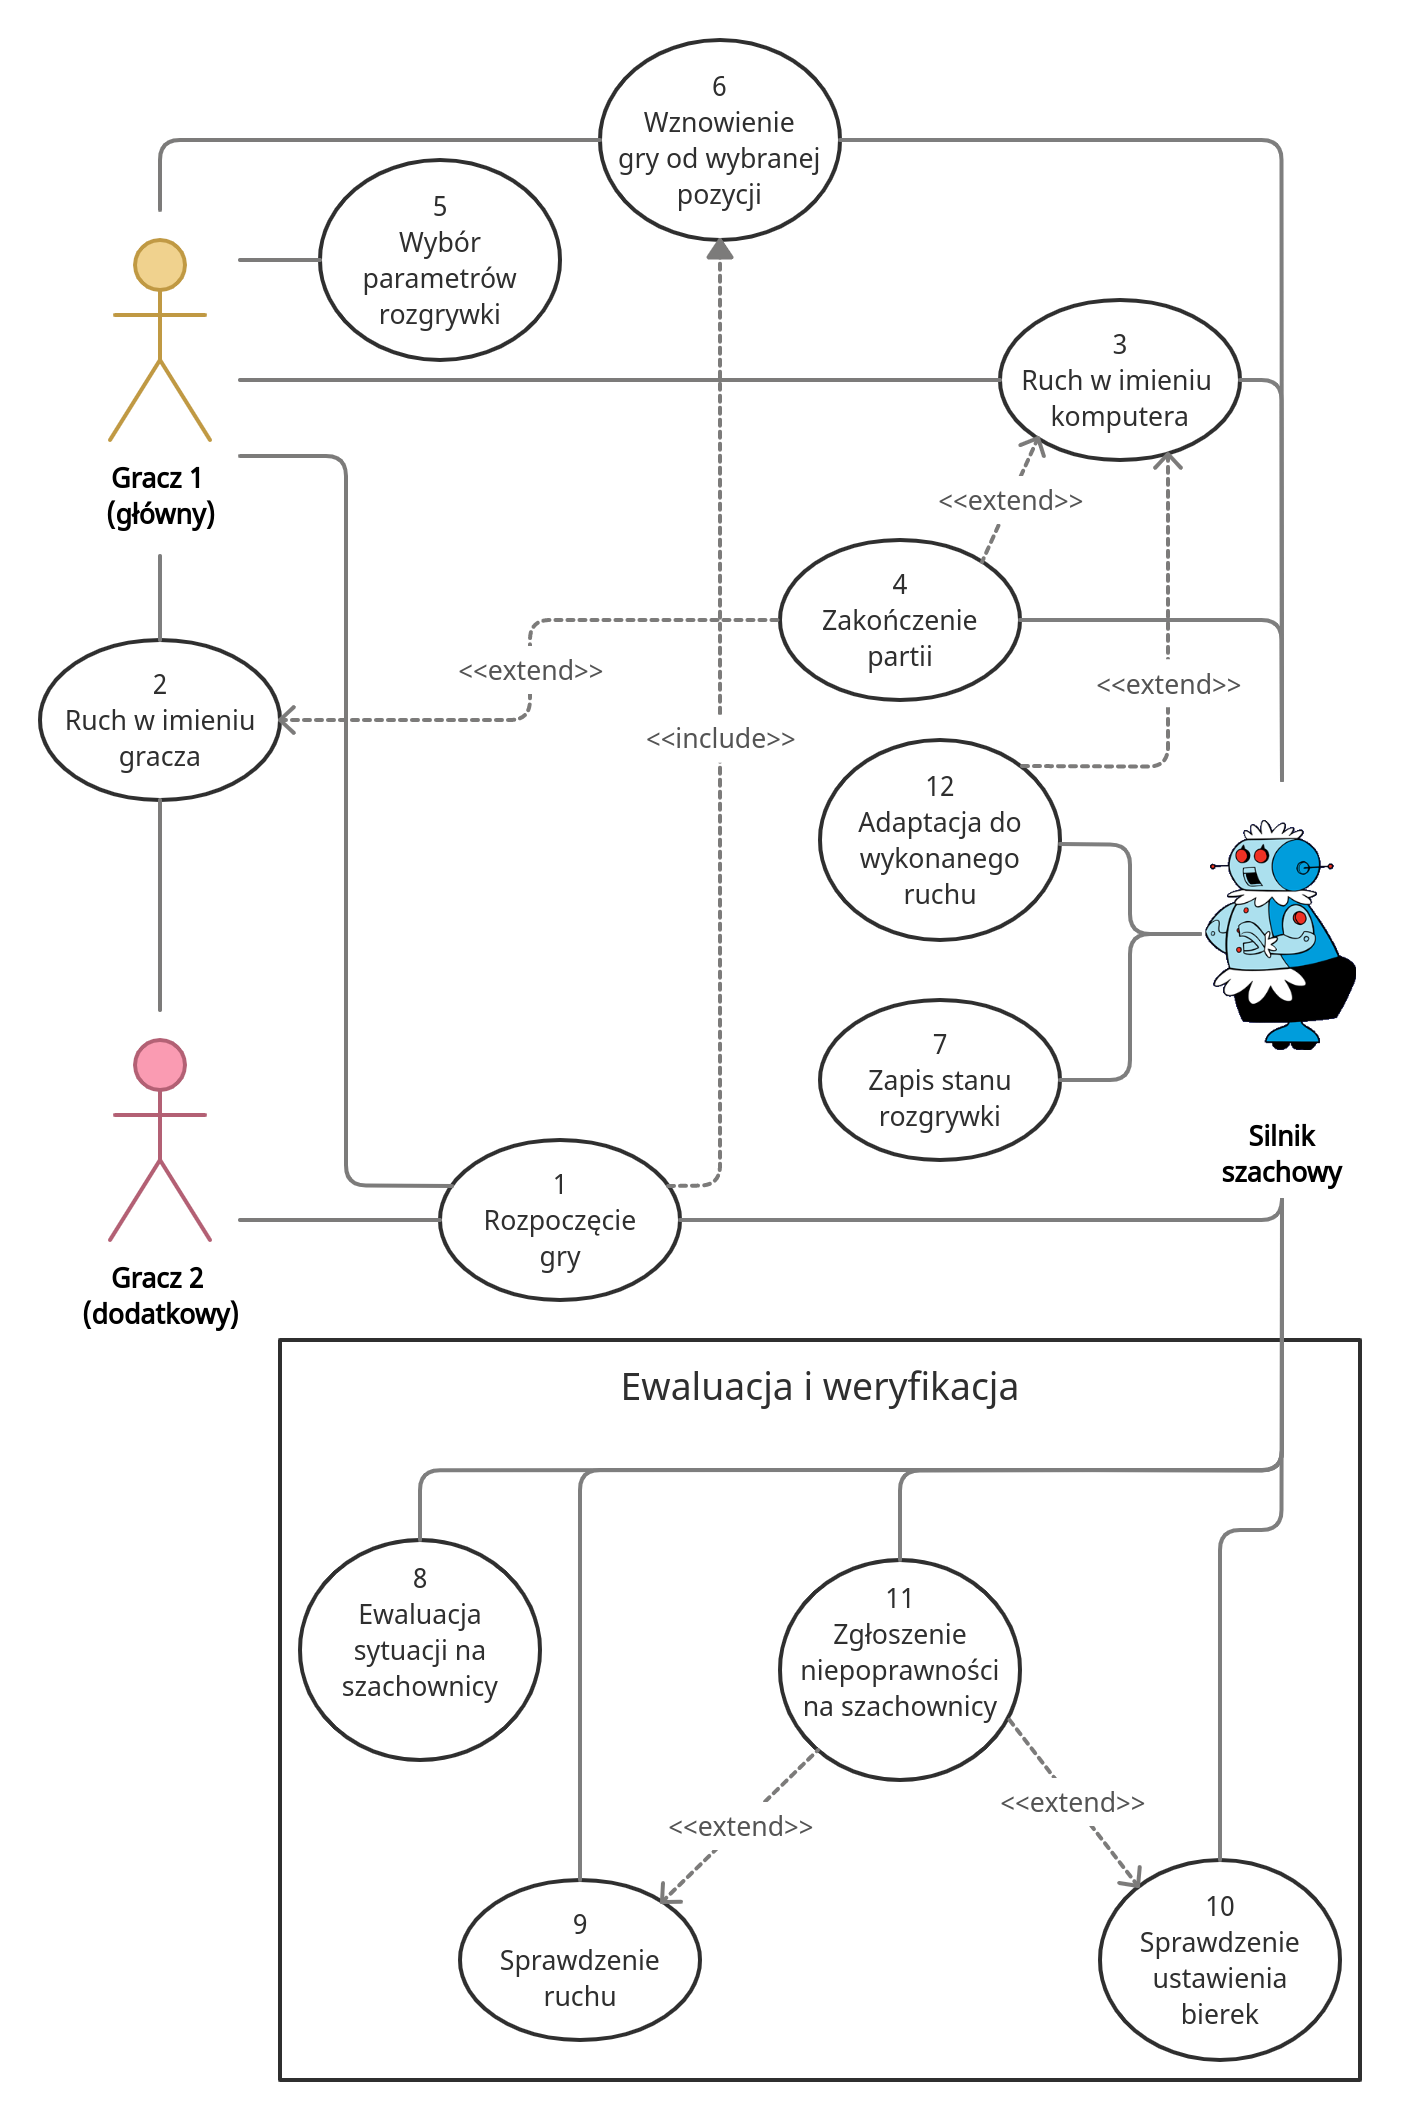
\includegraphics[width=0.9\textwidth]{diagram.png}
\end{document}
